\chapter{Wstęp}


%TODO to bym pominał. ok
Od kilku lat zauważalny jest trend ku autonomizacji jazdy samochodem.  
Ma to na celu wyeliminowanie czynnika, który jest najczęstszą przyczyną wypadków -- człowieka. Dodatkowym aspektem, który wpływa na rozwój przemysłu automotive, są koszty transportu. Zastosowanie autonomicznych ciężarówek poruszających się w konwojach znacząco zmniejszyłoby koszty logistyki dla firm spedycyjnych. %TODO mógłby Pan poszukać i dopisać też inne motywacje - ekonomia dzielenia itp.
Systemy, które wspomagają lub wręcz wyręczają kierowcę z obowiązku kierowania uwagi na samochód i jego otoczenie noszą miano ADAS (\textit{Advanced Driver Assistance Systems} -- zaawansowane systemy wspomagania kierowcy). 
W systemach wspomagających kierowcę stosuje się różne czujniki. Korzysta się z kamer pracujących w paśmie widzialnym i podczerwieni, radarów oraz lidarów. Radar oraz lidar działają na podobnej zasadzie, lecz korzystają z fal elektromagnetycznych o różnej długości.
Radar pracuje w paśmie mikrofal, natomiast lidar korzysta ze światła widzialnego.
 %TODO Inaczej. Opisać jakie czujniki się stosuje (krótko) i potem przejść do wizji. OK
Przykładowe systemy korzystające z przetwarzania obrazów to detekcja pasa ruchu lub wykrywanie zmęczenia kierowcy. 
Bardzo popularne jest stosowanie fuzji danych. 
Polega ona na jednoczesnym przetwarzaniu danych z dwóch lub więcej czujników, co zapewnia lepszą skuteczność algorytmu. Przykładem fuzji danych jest przetwarzanie danych z kamery i lidaru w tym samym czasie. %TODO to jest przykład - może być też fuzja z lidar albo 3 w 1.. OK
Na danych pozyskanych z kamery i radaru korzystają na przykład systemy aktywnego tempomatu lub detekcji pieszych.

%TODO A ogólnie to mógłby się Pan bardziej postarać :) :)

\section{Cele i założenia}

Celem niniejszej pracy było stworzenie aplikacji umożliwiającej testowanie algorytmów wizyjnych za pomocą symulatora ciężarówki.
Rozwiązanie to mogłaby być wykorzystane w ramach ćwiczeń laboratoryjnych poruszających problematyką systemów wizyjnych stosowanych w pojazdach autonomicznych prowadzonych w ramach kierunku Automatyka i Robotyka na Akademii Górniczo-Hutniczej.

\section{Istniejące systemy}
Aplikacje służące do testowania algorytmów wizyjnych są używane w przemyśle. 
Obecnie produkowane samochody są wyposażone w systemy, które bazując na widoku z kamery pomagają prowadzić samochód. 
Testowanie tych algorytmów jest niezwykle istotne, ponieważ niewykrycie błędów może prowadzić do katastrofalnych skutków, w tym potencjalnej śmierci człowieka. 
Przykładowo niewystarczające testowanie algorytmów w komercyjnym samochodzie Tesla 3 doprowadziło do śmiertelnego wypadku, ponieważ tzw. ,,autopilot'' nie wykrył poprawnie naczepy ciężarówki.

Popularne jest podejście do testowania SIL (ang. System in the loop - system w pętli), gdzie algorytm nie jest testowany w rzeczywistym pojeździe, lecz w oparciu o wcześniej nagrany przejazd samochodem testowym. Ocenie podlegają decyzje podejmowane przez algorytm w oparciu o nagranie video. Jest to rozwiązanie bezpieczniejsze oraz zdecydowanie tańsze. Wolumeny nagrań w bazach firm zajmujących się systemami ADAS sięgają milionów kilometrów jazd testowych.

\section{Zawartość pracy}

Rozdział drugi rozpoczyna się opisem poziomów autonomiczności samochodów. 
Ukazuje czym powinien charakteryzować się samochód, który znajduje się na określonym poziomie.
Następnie opisane są wybrane systemy wizyjne używane w branży automotive takie jak: detekcja pasa ruchu, detekcja świateł drogowych, wykrywanie znaków oraz detekcja samochodu poprzedzającego.
Opis jest opracowany na podstawie przeglądu publikacji naukowych.
Rozdział kończy krótki opis podstawowych operacji cyfrowego przetwarzania obrazów, których wyjaśnienie uznano za istotne z uwagi na ich częste stosowanie w systemach wizyjnych pojazdów autonomicznych.

Następny rozdział zawiera opis zrealizowanego systemu. 
Na początku dokonana jest ewaluacja dostępnych symulatorów jazdy wraz z uzasadnieniem wyboru Euro Truck Simulator 2. 
Kolejno opisana została architektura zaimplementowanej aplikacji. 
W~następnej części omówiono przykładowe algorytmy zaimplementowane w celu przetestowania i weryfikacji aplikacji stworzonej w ramach pracy. 
Końcowa część to sprawdzenie wydajności aplikacji w różnych sytuacjach.

Ostatni rozdział zawiera krótkie podsumowanie oraz ocenę przydatności aplikacji do prowadzenia zajęć dydaktycznych.

%TODO Proszę tych moich "TODO" nie usuwać, a jedynie oznaczać OK lub polemizować.
\chapter{Systemy wizyjne w pojazdach autonomicznych}

Współczesne pojazdy autonomiczne wykorzystują w~szerokim zakresie systemy wizyjne do analizy otoczenia. 
Jednym z pierwszych zastosowań algorytmów cyfrowego przetwarzania obrazów była detekcja pasa ruchu, która nie służyła do sterowania samochodem, lecz miała za zadanie wspomagać kierowcę w sytuacjach zmęczenia lub utraty koncentracji. 
Wraz z rozwojem technologii pojazdów autonomicznych, zaawansowanie systemów wizyjnych rosło od wspomnianej kontroli pasa ruchu, poprzez rozpoznawanie obiektów, które można spotkać na drogach: pieszych, pojazdów i rowerzystów, a także elementy infrastuktury: znaków i świateł drogowych.
%TODO ująłbym szerzej, że obiektów: pieszych, rowerzystów, pojazdów itp. OK
%TODO styl. zbyt zamotane zdanie. OK - usunięte
W kolejnych podrozdziałach zostaną opisane czujniki stosowane w przemyśle motoryzacyjnym. Następnie zawarty jest krótki opis poziomów autonomiczności pojazdów. Rozdział kończy opis działania algorytmów wizyjnych w samochodach.

%TODO dodałbym podrozdzialik o czujnikach zbudowany wokół analizy rysunku 2.1. (brakuje tej treści) OK - zrobione niżej
%TODO Inna sprawa, że w kolejnych podrozdziałch... to trzeba wymienić, że te czujniki, potem poziomy, a potem systemy wizyjne.

\section{Poziomy autonomiczności}

Całość systemów, które wspomagają kierowcę w trakcie jazdy nazwano ADAS (\textit{Advanced Driver Assistance Systems}). 
Aby usystematyzować i podzielić poziom wpływu systemów na sterowanie pojazdem wprowadzono poziomy autonomiczności jazdy.

\begin{figure}
  \centering
  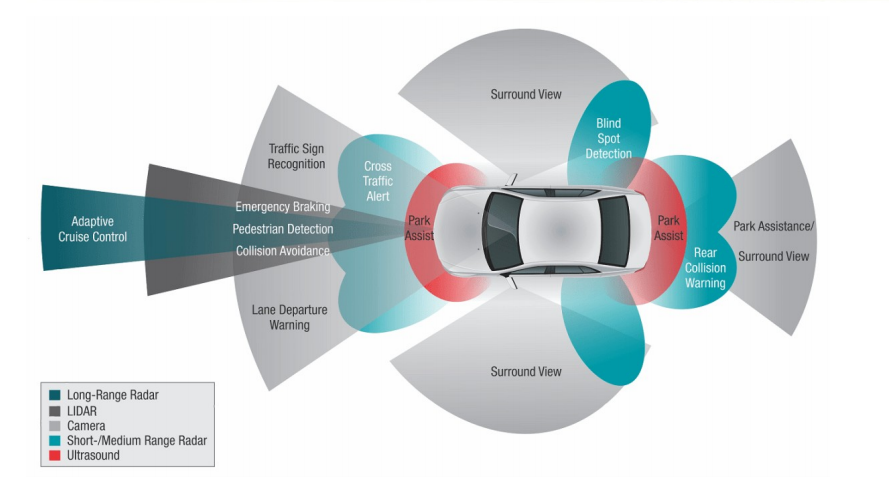
\includegraphics[width=13cm]{img/systemy_autonomiczne_ogolnie.png}
  \caption{Ogólny schemat kamer i radarów we współczesnych pojazdach autonomicznych\cite{S1}}
  \label{fig:kamery_i_radary}
  % https://aindustryreports.com/2019/05/23/advanced-driver-assistance-system-sensor-market-technological-innovations-in-north-america-to-boost-regional-market-attractiveness-through-2026/
\end{figure}

Na rysunku \ref{fig:kamery_i_radary} daje się zauważyć znaczna liczba kamer i radarów wspomagająca kierowcę. Z przodu i tyłu pojazdu umieszczone są czujniki ultradźwiękowe (oznaczone na czerwono), których zadaniem jest wspomaganie procesu parkowania samochodu poprzed wykrywanie obiektów w bliskim otoczeniu pojazdu.
Pozostając przy parkowaniu, kamera umieszczona z tyłu pojazdu również wspomaga parkowanie. Co raz popularniejsze są systemy czterech kamer po jednej na każdą krawędź samochodu. Na podstawie obrazu pochodzącego z nich generowany jest obraz samochodu z lotu ptaka.
Kamery są również używane w systemie asystenta pasa ruchu i detekcji i rozpoznawania znaków drogowych.
Radary bliskiego zasięgu (jasnozielony )i lidary (ciemnoszary) znalazły zastosowanie w komponentach odpowiedzialnych za sytuacje awaryjne takie jak system unikania kolicji czy detekcja martwego pola.
Radar dalekiego zasięgu jest używany w tempomacie adaptacyjnym.
Powszechną techniką jest stosowanie redundancji w krytycznych systemach, co jest regulowane poprzez normy bezpieczeństwa ISO 26262.
%TODO uwaga j.w. + nie byłbym przekonany, że istnieje coś takiego jak normy ADAS. Są oczywiście normy bezpieczeństwa systemów - słynne ISO 26262 OK

%TODO Przydałoby się podać na podstawie czego opracowana została ta klasyfikacja SAE - źródło

\subsection{Poziom zerowy -- brak autonomiczności}

Obecnie większość samochodów na drodze zalicznanych jest do tego poziomu. %TODO zaliczanych jest do tego poziomu ? -OK
Samochód jest w pełni kontrolowany przez człowieka, chociaż mogą pojawiać się proste systemy, które mogą pomóc kierowcy np. system awaryjnego hamowania. 
Dopóki bezpośrednio nie wpływa on na tor jazdy, nie jest to system autonomiczny. 
Innym przykładem jest ABS (\textit{Anti-lock brake system} -- system zapobiegający blokowaniu kół podczas hamowania), który również nie jest systemem, który zapewniałby autonomiczność pojazdowi. %TODO rozwinąc skrót ABS, powt system - OK
Służy on poprawie bezpieczeństwa i jego działanie opiera się tylko na odczycie danych z czujników niezależnie od aktualnej sytuacji na drodze i wokół pojazdu. System zadziała poprawnie na drodze asfaltowej w przypadku awaryjnego hamowania i pozwoli bezpiecznie ominąć przeszkodę. Praktyka pokazuje, że w przypadku, gdy zajdzie potrzeba nagłego zatrzymania samochodu na oblodzonej drodze lepiej jest, aby system ABS nie zadziałał, ponieważ znacząco wydłuża drogę hamowania. Jako, że samochody poziomu zerowego nie interpretują stanu otoczenia, wspomniany system będzie działał zawsze, niezależnie od tego czy przyniesie to pozytywny efekt. %TODO może Pan bardziej konkretnie napisać o tym (treść) - OK (opisać pozostałe systemy - ESP itd.?)


\subsection{Poziom pierwszy -- asystenci jazdy}
%TODO używa Pan słowa "asysta", a mi ono nie pasuje: https://sjp.pwn.pl/sjp/asysta;2441704.html
%TODO wspomaganie ?
%to jest kalka z angielskiego, gdzie mamy "driver assists". W polskim pojawiają się asystenci jazdy (jako systemy wspomagające kierowcę), którzy jak rozumiem pełnią asystę. Zmieniam na asystenci jazdy, oczywiście do ew. zmiany

Jest to najniższy poziom autonomiczności. 
Auto posiada pojedynczy system wspomagania kierowcy, taki jak zmienianie kierunku jazdy samochodu lub przyspieszanie (tempomat). 
%TODO tutaj to słowo "sterowanie" jest mylące. Proszę to jakoś inaczej ująć. Albo podać przykład, bo asystet pasa ruchu chyba też się tu mieści OK
Przykładem systemu, który jest montowany w samochodach autonomicznych poziomu pierwszego jest adaptacyjny tempomat, czyli system, który zachowuje bezpieczny dystans od poprzedzającego pojazdu. Kierowca kontroluje pozostałe aspekty jazdy samochodem takie jak kierowanie i hamowanie. %TODO przerobić na przykładem.... OK

\subsection{Poziom drugi -- częściowa automatyzacja jazdy samochodem}
Oznacza zaawansowanych asystentów jazdy. %TODO asysty j.w do ew. zmiany OK
Samochód może sam kontrolować zarówno kierunek jazdy i przyspieszanie oraz hamowanie. %TODO tu może zamiast sterowanie - kierunek jazdy, bo kontrolować sterowanie średnio brzmi  OK
Jest w stanie jechać samodzielnie, lecz wymaga ciągłej obecności kierowcy za kierownicą, który może w~każdej chwili przejąć kontrolę nad samochodem. 
Obecnie stosowane systemy jazdy autonomicznej takie jak np. Tesla Autopilot montowane w samochodach marki Tesla (rys. \ref{fig:teslas}) kwalifikują się jako poziom drugi.

\begin{figure}
  \centering
  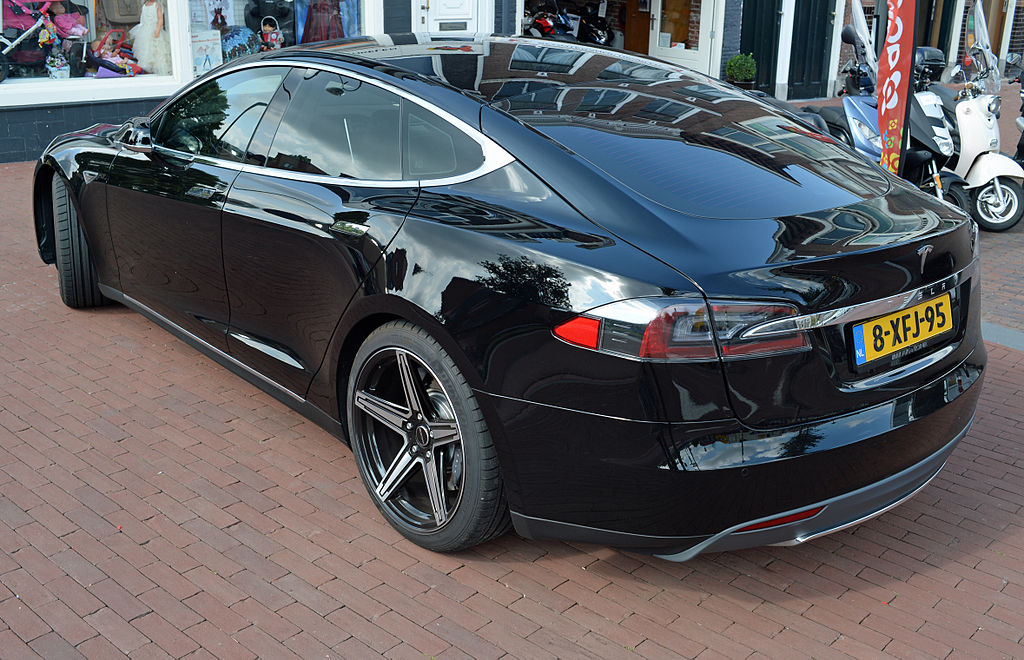
\includegraphics[width=12cm]{img/tesla.jpg}
  \caption{Tesla Model S -- pierwszy samochód z drugim poziomem zaawansowania systemów wspomagania kierowcy (\textit{źródło: Wikipedia})}
  \label{fig:teslas}
  % https://pl.wikipedia.org/wiki/Tesla_Model_S#/media/Plik:2014_Tesla_Motors_Model_S_(rear_view)_Netherlands.jpg
\end{figure}
%TODO odniesnie do rysunku w tekście. OK

\subsection{Poziom trzeci}

Poziom trzeci mocno opiera się na poziomie drugim. %TODO styl. jakoś inaczej trzeba tą myśl ująć, bo to źle wygląda jako początek zdania. OK
Samochód posiada możliwość percepcji otaczającego go środowiska i~na podstawie zgromadzonych informacji samodzielnie podejmować decyzje. %TODO detekcji - percepcji OK
System jest jednak wciąż zależny od człowieka, który musi pozostać czujny i być w stanie zareagować, gdy system nie będzie w stanie podjąć decyzji. 
W~2019r. Audi wprowadziło model A8, który zapowiadano jako pierwszy samochód poziomu trzeciego. 
System \textit{Traffic Jam Pilot} bazując na danych z lidaru oraz kamer zapewniał autonomiczną jazdę w korkach. 
Problemem okazał się brak odpowiednich regulacji prawnych. %TODO może brak odpowiednich regulacji prawnych OK
W Stanach Zjednoczonych stosowanie tego systemu było zabronione, więc samochód w okrojonej wersji sprzedawano jako pojazd autonomiczny drugiego poziomu. 
Na rynku europejskim samochód pojawił się z zaimplementowaną funkcjonalnością asystenta jazdy w korku. %TODO sprawdzał Pan w jakich krajach ? -Wiem, że wariant europoejski ma tę funkcjonalność (pewne źródło: Aptiv :).

\subsection{Poziom czwarty}

Poziom czwarty zapewnia poprawną reakcję samochodu w nagłych sytuacjach takich jak np. wypadek lub pęknięcie opony. %TODO trochę niejasne -OK
Pojazdy nie wymagają ingerencji człowieka w znakomitej większości sytuacji, jednak kierowca zawsze powinien być w stanie przejąć kontrolę. 
Podobnie jak w poziomie trzecim problemem okazały się ograniczenia prawne. 
Samochody te mogą z reguły poruszać się na ograniczonym obszarze. 
Obecnie w fazie testów są samochody takie jak Waymo lub NAVYA.

\subsection{Poziom piąty - pełna autonomia}
Samochody nie wymagają ingerencji ze strony człowieka. 
Najprawdopodobniej nie będą wyposażone w kierownicę ani pedały. 
Będą w stanie jechać gdziekolwiek, system sterowania będzie działał na poziomie doświadczonego kierowcy. 
Samochody te są obecnie w stanie wczesnych testów, jednak można się spodziewać, że w ciągu najbliższych kilkunastu lat pierwsze w pełni autonomiczne samochody będą pojawiać się na drogach.
%TODO tu akurat byłbym ostrożny,., -W stanach były z tego co kojarzę autonomiczne UBERy, któryś miał wypadek nawet. A ostatnio Aptiv miał mieć przejazd samochodu po A4 z kierowcą tylko ze względów prawych.. ale nie wyszło też ze względów prawnych.

\subsection{Autonomiczne samochody ciężarowe}

Warto zaznaczyć, że ważnym polem do zastosowania systemów autonomicznej jazdy jest transport ciężarowy. %TODO konkretniej, bo transport to też auta osobowe OK
Systemy wspomagające kierowcę pojawiają się w samochodach ciężarowych analogicznie do samochodów osobowych. %TODO ale niejasne gdzie  OK
W najbliższych latach planuje się rozwijanie koncepcji autonomicznych samochodów ciężarowych poprzez tworzenie konwojów, w których kierowca znajduje się tylko w pierwszym samochodzie (źródło: \cite{W4})%TODO powt. ciężarówek - lepiej sam. ciężarowy. Przydałoby się źródło (choćby on-line). OK
Kolejnym krokiem będzie autonomiczna jazda na dystansie trasy ze wsparciem kierowcy podczas załadunku i rozładunku. 
Ostatnim krokiem, podobnie jak w przypadku samochodów osobowych, będzie w pełni autonomiczna jazda bez udziału człowieka.

Systemy wizyjne stosowane w ciężarówkach nie odbiegają sposobem pracy od tych używanych w samochodach osobowych.


%TODO To by przydało się ująć jedak jako \section, dwa zdania wstępu i potem \subsection dla poszczególnych systemów. Tak jak jest teraz to dziwnie wygląda.

%TODO Tak sobie jeszcze myślę, że oprócz metody konkruencyjnej dobrze by było opisać przykład metody deep AI. Bez istotnych szczegółów, ale pokazać, że tak też się ten problem rozwiązauje.


\section{Algorytmy wizyjne w pojazdach autonomicznych}
W~kolejnych podrozdziałach zostaną opisane algorytmy wizyjne, których zadaniem jest analiza otoczenia samochodu. %TODO detekcja otoczenia dziwnie brzmi. OK
W ostatnich latach dynamicznie rozwijającą się dziedziną w systemach wizyjnych i motoryzacji są sieci neuronowe, które są obecnie najczęściej wybierane do implementacji w samochodach. 
Jednakże ze względu na edukacyjny charakter pracy opisane zostaną algorytmy bazujące na klasycznych metodach przetwarzania obrazach cyfrowych. %TODO mógłby Pan to nieco rozwinąć - to i wątek NN 
W niektórych metodach zostaną użyte proste techniki uczenia maszynowego.
%TODO To do tego wstępu rozdziału OK
\subsection{Wykrywanie pasa ruchu}

\label{sec:lane_detection}

Wykrywanie pasa ruchu było jednym z pierwszych algorytmów implementowanych w samochodach komenrcyjnych. %TODO niejasne przez kogo OK
W trakcie jazdy kluczowym elementem jest utrzymanie samochodu w pasie jezdni niezależnie od stanu nawierzchni, pogody, czy prędkości (rys. \ref{fig:inputimg1}).

\begin{figure}
  \centering
  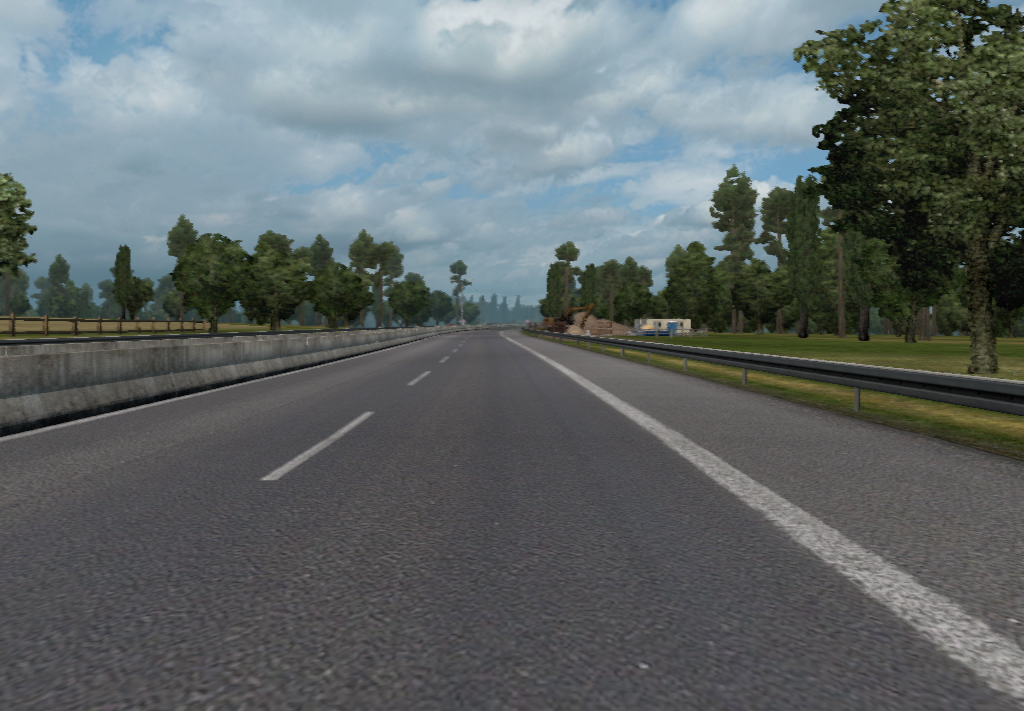
\includegraphics[width=7cm]{img/input.png}
  \caption{Przykładowy obraz wejściowy algorytmu detekcji pasa ruchu}
  \label{fig:inputimg1}
  \end{figure}
%TODO odnośnik do rysunku + może zamiast jednego mega kilka (4) mniejsze pokazujące różne warunki.

W~najczęstszym przypadku wejściem do algorytmu jest obraz z kamery umieszczonej pod pewnym kątem do nawierzchni zamontowanej w okolicy przedniego zderzaka, atrapy chłodnicy lub za lusterkiem wstecznym. %TODO myślę, że za luterkiem też. OK
W niniejszej pracy, większość przetwarzanych obrazów pochodzi z symulatora Euro Truck Simulator 2, (który dokładniej jest opisany w rozdziale \ref{sec:ets2}), gry komputerowej, która posiada zaawansowaną grafikę, która przypomina otaczającą rzeczywistość, a także udostępnia możliwości programistyczne, które ułatwią stworzenie aplikacji do testowania algorytmów wizyjnych, co jest założeniem niniejszej pracy. %TODO odnośnik to opisu tego Euro Truck z drugiej części pracy OK

W niniejszym podrozdziale zostanie opisany algorytm z artykułu \cite{T3}. %TODO "sekcja" to nie jest polskie słowo na rozdział/podrozdział. OK
Autor korzysta w nim z podstawowych operacji przetwarzania obrazów. 



\begin{figure}
  \centering
  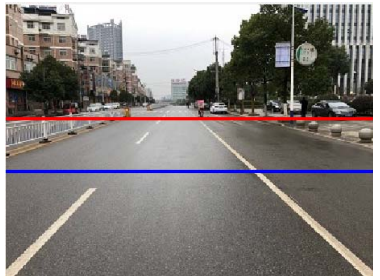
\includegraphics[width=10cm]{img/roi.png}
  \caption{Linie obrazujące granice obszaru poddawanego analizie\cite{T3}}
  \label{fig:roi}
  % artykuł
\end{figure}

Pierwszym krokiem jest wyodrębnienie z obrazu ROI \footnote{ROI (ang.) -- \textit{Region of Interest} -- obszar obrazu poddawany analizie i dalszemu przetwarzaniu} (rys. \label{fig:roi}). %TODO odnośnik do rysunku OK
Ma to na celu ograniczenie ilości danych poddawanych analizie, a co bardziej istotne odrzuca te fragmenty obrazu, na których na pewno nie będzie jezdni (powyżej czerwonej linii), a także te gdzie obraz linii mógłby być zakłócony. 
Warto zauważyć, że pomiędzy liniami - czerwoną i niebieską znajduje się prawie dwa razy więcej długości drogi niż w obszarze pod niebieską linią. Obszar pod niebieską linią jest odrzucany, ponieważ na dużym obszarze obrazu znajduje się niewielki fragment jezdni, co może generować problemy z poprawną detekcją w przypadku linii przerywanej.
%TODO a jaki jest argument dlaczego nie przed niebieską ? OK

Kolejnym etapem jest ekstrakcja linii rozdzielającej pasy. %TODO no to nie pasów, tylko linii rozdzielająych pasy OK
W większości krajów mają one kolor biały, rzadziej żółty. 
Są to kolory, które na drodze inną funkcję niż barwa znaków poziomych, w tym linii. %TODO styl.  OK
Mając na wejściu obraz RGB\footnote{RGB -- obraz o~trzech składowych barwnych: czerwonej (R), zielonej (G) i~niebieskiej (B)} można zauważyć, że składowe czerwona i zielona mają większe wartości tam gdzie na obrazie są linie w porównaniu do niepomalowanej nawierzchni jezdni. %TODO standardowa nawierzchnia OK
W~omawiany artykule zaproponowano następującą metodę segmentacji linii:
\begin{equation}
\label{eq:IMij}
IM(i,j)=\left\{\begin{matrix}
255, & \begin{matrix}
R(i,j)\geq (0.2R_{min}+0.8R_{max})\\ 
G(i,j)\geq (0.2G_{min}+0.8G_{max})
\end{matrix}\\ 
0, & wpp.
\end{matrix}\right.
\end{equation}
%TODO u mnie ten footnote nie działa. u mnie również. Ciężko w Latex wstawiać przypisy w równaniach - może uznamy, że skrót jest powszechnie znany w środowisku?

\begin{equation}
\label{eq:Gij}
G(i,j)=\left\{\begin{matrix}
255, & \begin{matrix}
R(i,j)\geq G(i,j) \geq B(i,j)\\ 
IM(i,j)>0
\end{matrix}\\ 
0, & wpp.
\end{matrix}\right.
\end{equation}

\begin{equation}
\label{eq:Gray}
Gray(i,j)=R(i,j)+G(i,j)-2B(i,j)+0.3*8|R(i,j)+G(i,j)|
\end{equation}

\begin{equation}
\label{eq:GMij}
GM(i,j)=\left\{\begin{matrix}
128, &  Gray(i,j)\geq 0.8*Gray_{m} \\ 
255, & \begin{matrix}
2*Gray_{avg} \leq Gray(i, j) \leq Gray_{m}\\albo\\ 
G(i,j)=255
\end{matrix} \\ 
0,   & wpp.
\end{matrix}\right.
\end{equation}

W~równaniu \eqref{eq:IMij} \ ${IM(i,j)}$ oznacza tymczasową macierz cech koloru. ${R(i,j)}$ oznacza wartość składowej czerwonej, a~${G(i,j)}$ składową zieloną. 
${R_{max}}$, ${R_{min}}$, ${G_{max}}$, ${G_{min}}$ reprezentują maksymalną i ~inimalną wartość składowej czerwonej, a także maksymalną i~minimalną wartość składowej zielonej. 
W~równaniu \eqref{eq:Gray} \ $ Gray(i,j)$ oznacza obraz wejściowy w skali szarości, na wartości którego ma wpływ każda ze składowych barwnych. 
W~ostatnim równaniu \eqref{eq:GMij} \ $GM(i,j)$ oznacza obraz wynikowy, na którym zaznaczone jest wysegmentowane poziome oznaczenie jezdni. 
$Gray_{avg}$ to średnia wartość obrazu w skali szarości w danym wierszu, natomiast $Gray_{m}(i,j)$ oznacza wartość maksymalną dla danego wiersza.

\begin{figure}
  \centering
  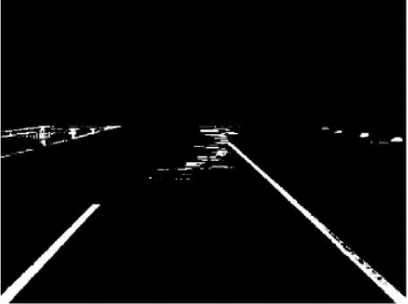
\includegraphics[width=7cm]{img/segmentacja.png}
  \caption{Obraz $GM$ -- wysegmentowane linie\cite{T3}}
  \label{fig:segmented}
\end{figure}


Kolejnym etapem opisywanego algorytmu jest wykrywanie krawędzi zrealizowane za pomocą filtru Canny'ego. 
Jest to filtr nieliniowy z histerezą, który dobrze sprawdza się do wykrywania krawędzi na obrazach niejednorodnych i~rozmytych. 
Następnie podejmowana jest ekstrakcja cech linii. 
Na potrzeby wyjaśnienia działania podanego fragmentu algorytmu przyjęto:
\begin{itemize}
\item $IME$ -- obraz z równania \eqref{eq:GMij} po filtracji filtrem Canny'ego
\item $IMC$ -- obraz $GM$ z równania \eqref{eq:GMij}
\end{itemize}

Dla każdego piksela w~obrazie $IME$, który został oznaczony jako krawędź, zostaje sprawdzona następująca zależność:
\begin{equation}
	\begin{matrix}
	IMC(i,j+1)+IMC(i,j)+IMC(i,j-1)+IMC(i-1,j+1)\\
	+IMC(i-1,j)+IMC(i-1,j-1)+IMC(i+1,j+1)+IMC(i+1,j-1)>0
	\end{matrix}
\end{equation}
Jeśli jest ona spełniona, wybrany punkt na obrazie $IME$ zostaje uznany jako krawędź pasa jezdni.
%TODO Napisać co to oznacza w praktyce OK
W praktyce ma to za zadanie zwiększyć skuteczność algorytmu. Linie oddzielające pasy ruchu z reguły mają na obrazie szerokość większą niż jeden piksel (a taką szerokość mają póki co na obrazie uzyskanym po detekcji krawędzi), więc jeśli choć jeden piksel z ośmiopikselowego otoczenia jest uznawany za krawędź, to rozważany piksel również jest traktowany jako element krawędzi.

\begin{figure}
  \centering
  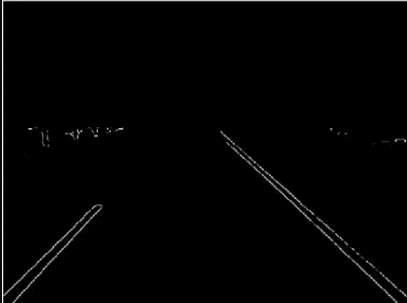
\includegraphics[width=7cm]{img/canny.png}
  \caption{Obraz po zastosowaniu filtra Canny'ego oraz ekstrakcji cech linii\cite{T3}}
  \label{fig:canny}
\end{figure}

Do ostatecznego wykrycia linii prostych należy użyć zmodyfikowanej transformaty Hougha( \textit{constraint Hough transform}). 
Główna różnica pomiędzy wykorzystywaną, a klasyczną transformatą Hougha polega na tym, że wartości $\rho$ i $\theta$ są skwantowane i pogrupowane. 
Dzięki takiej modyfikacji nieidealnie proste linie lub takie, które leżą blisko siebie nie będą wykryte wielokrotnie. %TODO styl. zdania... OK

\begin{figure}
  \centering
  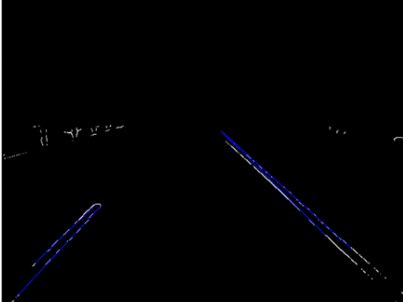
\includegraphics[width=7cm]{img/prehough.png}
  \caption{Wynik algorytmu detekcji linii\cite{T3}}
  \label{fig:result}
\end{figure}


%TODO Dlaczego zakomentowane ? Artykuł, na którym to jest oparte zawierał pewne luki i nie byłem w stanie dociec o co tak naprawdę autorom chodzi

%\subsection{Detekcja zakrętów}
%Podobnym zadaniem jest detekcja pasa ruchu w zakręcie. Kształt zakrzywionej linii może być opisany za pomocą paraboli z równania \ref{eq:ld_1}. Zauważono, że fragment drogi bliżej samochodu z reguły jest prosty, zakrzywienie widać powyżej pewnej odległości, a na obrazie powyżej pewnej wysokości. Równanie \ref{eq:ld2} pokazuje model pasa ruchu, gdzie $y_m$ to współrzędna punktu, w którym prosta przechodzi w krzywą.
%\begin{equation}
%x=a+by+cy^{2}
%\end{equation}
%
%\begin{equation}
%x=\begin{cases}
%a+by,\qquad\qquad y\leq y_{m}\\ c+dy+ey^{2},\qquad y > y_{m} \end{cases}
%\end{equation}
%
%gdzie ponadto:
%\begin{itemize}
%\item $a,b$ -- parametry linii
%\item $c,d,e$ -- parametry krzywej
%\end{itemize}
%
%Linie prosta i krzywa powinny spotykać się w jedym punkcie, którego współrzędna wysokościowa jest równa $y_m$. Po pewnych przekształceniach otrzymano równanie \ref{eq:ld_3} i \ref{eq:ld_4}.
%
%\begin{equation}
%a+by_{m}=c+dy_{m}+ey_{m}^{2}
%\end{equation}
%
%\begin{equation}
%b = d+2ey_m
%\end{equation}
%
%Ostatecznie uzyskano zależność \ref{eq:ld_5} pomiędzy parametrami krzywych.
%
%\begin{equation}
%\begin{cases} c=a+\frac{y_{m}}{2}(b-d) \\
%e=\frac{1}{2y_{m}}(b-d) \end{cases}
%\end{equation}

%TODO Dla zwiększenia objęctości

\subsection{Detekcja znaków drogowych}

Innym w swojej naturze zadaniem stawianym przed systemami wizyjnymi w pojazdach autonomicznych jest detekcja i rozpoznawanie znaków drogowych. %TODO i rozpoznawanie OK
Systemy tego typu pojawiały się dość wcześnie w~samochodach pełniąc jedynie funkcję ostrzegawczo-informacyjną.
Coraz bardziej dynamicznie rozwijające się systemy wspomagające kierowcę wymagają od podsystemu odpowiedzialnego za detekcję znaków drogowych dużej skuteczności, ponieważ na ich efektach pracy opierają decyzje o sterowaniu pojazdem. %TODO podsystem... powt. detekcja OK
W przypadku tego zagadnienia istotnym problemem jest brak ujednoliconego zestawu znaków dla całego świata. %TODO w przypadku tego zagadnienia OK
Obecnie każdy kraj posiada swój zestaw znaków, które w ogólności są podobne, jednak różnice w szczegółach komplikują projektowanie opisywanych systemów. %TODO może komplikują projetkowanie OK
Proponowanym rozwiązaniem jest zbudowanie odpowiednio dużej bazy wzorców znaków i~stosowanie określonego zestawu w zależności od konkretnej lokalizacji. 

Rozwiązanie proponowane w~pracy \cite{T2} składa się z dwóch etapów. 
Pierwszy to detekcja znaku, a drugi to jego klasyfikacja. 
Do wykrycia znaku drogowego na obrazie pochodzącym z kamery umieszczonej w samochodzie użyto metody \textit{Radial Symmetry Transform} do detekcji znaków ograniczenia prędkości. 
Obecnie stosowane metody detekcji znaków drogowych bazują na segmentacji koloru lub ekstachowania cech kształtu. %TODO zdanie niejasne OK

\subsubsection{Symmetry Transform}

Klasyczne detektory kształtu wymagają często zamkniętych konturów. 
Techniki odporne, takie jak transformata Hougha dla okręgów wymaga dużych nakładów obliczeniowych dla dużych obrazów. 
Metoda \textit{\textit{fast radial symmetry detector} -- (ang. szybki detektor symetrii radialnej) -- FRSD} może być używana w~czasie rzeczywistym. %TODO a to nie powinno być detektor symetrii radialnej ? OK
Znakomita większość znaków z ograniczeniem prędkości to koło z czerwonym brzegiem i wartością ograniczenia w środku na białym tle. 
Opisywana metoda detekcji jest kompatybilna ze wszystkimi głównymi metodami klasyfikacji takimi jak np. SVM (ang. \textit{Support Vector Machine} -- maszyna wektorów wspierających). 
Zaletą użycia opisywanego algorytmu jest fakt, że wraz z informacją o wykrytym znaku podawana jest skala znaku, co znacząco ułatwia klasyfikację, ponieważ niepotrzebne staje się używanie szablonów o wielu rozmiarach dla wielu różnych rozdzielczości. %TODO nie wiem czy główną, czy dodatkową. Ponadto proszę spróbować mniej słowa "metoda". OK

Detektor radialnej symetrii jest wariantem transformaty Hougha dla okręgów. 
Jest on wykonywany w porządku $kp$, gdzie $k$ oznacza liczbę promieni, które są szukane, a~$p$ liczbę pikseli. Stanowi to różnicę w stosunku do klasycznej transformaty Hougha wykonywanej w porządku $kbp$, gdzie każdy piksel na obrazie krawędzi ,,głosuje'' dla każdego koła z dyskretnego zestawu promieni. $b$ oznacza dyskretyzację zestawu promieni okręgów, które mogą przechodzić przez aktualnie analizowany punkt.

\begin{figure}
  \centering
  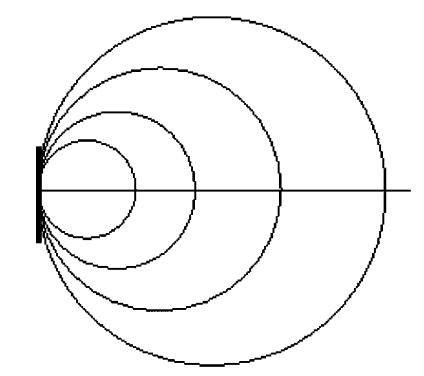
\includegraphics[width=7cm]{img/fsrd1.png}
  \caption{Algorytm głosowania - dla danego punktu krawędzi środki rodziny krawędzi leżą na lini prostopadłej do krawędzi\cite{T2}}
  \label{fig:frsd1}
\end{figure}

FRSD eliminuje czynnik $b$ poprzez pozyskanie informacji o kierunku gradientu z detektora krawędzi Sobela.
Zamiast sprawdzania każdego możliwego kierunku promienia, sprawdzany jest jedynie kierunek prostopadły do kierunku gradientu, co jest widoczne na rysunku \ref{fig:frsd1}. 
Powoduje to, że przestrzeń rozwiązań z~trójwymiarowej staje się dwuwymiarowa, co pozwala na używanie algorytmu w czasie rzeczywistym. 
Operacja detekcji symetrii radialnej może być prosto zrozumiana jako rozważenie wszystkich możliwych okręgów, których dany piksel może być częścią, jeżeli znany jest kierunek krawędzi, to okręgi są szukane tylko na linii prostopadłej do krawędzi (rys. \ref{fig:frsd1}). %TODO to może dać obok tego poprzedniego rysunku. detekcja symetrii radialnej OK



\begin{figure}
  \centering
  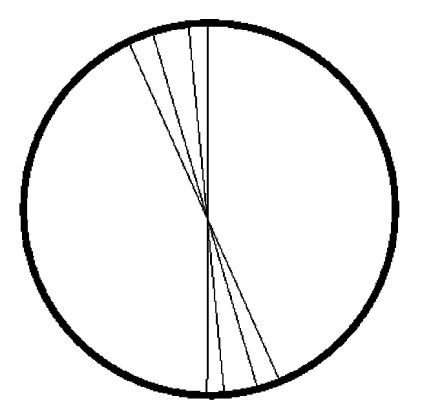
\includegraphics[width=7cm]{img/fsrd2.png}
  \caption{Działanie FRSD dla okręgu, zauważalne przecięcie średnic skutkuje istnieniem maksimum lokalnego w środku okręgu.\cite{T2}} %TODO Zachowanie - działanie OK
  \label{fig:frsd2}
\end{figure}
Na rysunku \ref{fig:frsd2} widać działanie algorytmu dla okręgu. Badanie wartości gradientu tylko na kierunku prostopadłym do orientacji gradientu implikuje istnienie maksimum w środku okręgu.


Praktyczna realizacja jest wykonywana na obrazie cyfrowym, więc promień jest skwantowany na kilka przedziałów długości. %TODO niejasne OK
Istotne jest poprawne dobranie ograniczeń na długość promienia. 
Na rysunku \ref{fig:tsd} po prawej stronie jest widoczny znak ograniczenia prędkości, który powinien zostać wykryty. 
Daje się zauważyć, że można dobrać odpowiednie zakresy promienia dla znaków, które będą pojawiać się na obrazie z kamery. Można również wyodrębnić obszar, na którym znaki na pewno nie będą się pojawiać (jezdnia przed pojazdem, wyższa część nieba). %TODO to zdanie jest takie dziwne - pełna zgoda OK
\begin{figure}
  \centering
  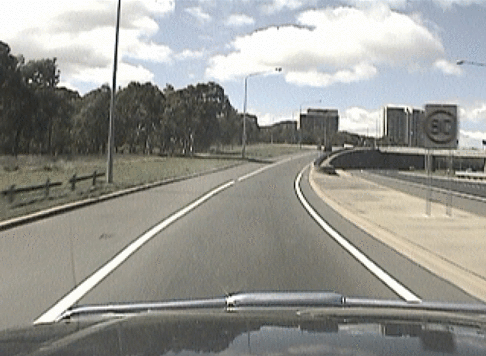
\includegraphics[width=7cm]{img/znaki1.png}
  \caption{Obraz wejściowy algorytmu detekcji znaków drogowych\cite{T2}}
  \label{fig:tsd}
\end{figure}

%\begin{figure}
%\centering
%\subfloat[obraz 1]{\label{fig:znaki2}
%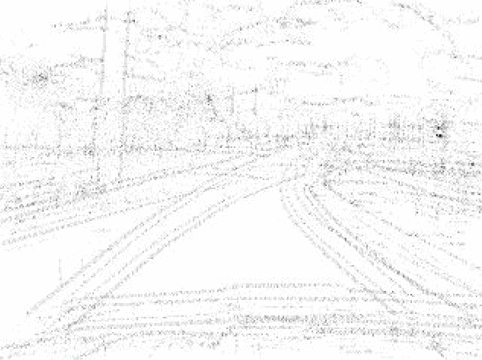
\includegraphics[width=0.3\textwidth]{img/znaki2.png}}
%\quad
%\subfloat[obraz 2]{\label{fig:znaki3}
%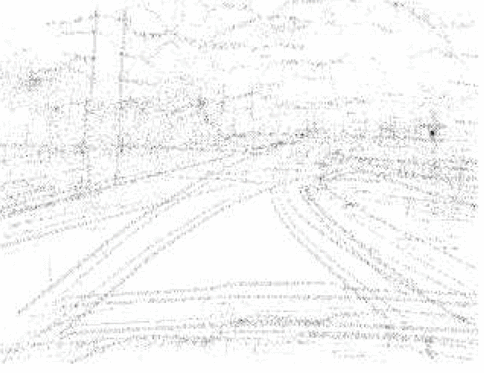
\includegraphics[width=0.3\textwidth]{img/znaki3.png}}
%\caption{Wyniki detekcji, gdy zakres promieni jest zbyt mały \protect\subref{subfigure_a} i zbyt duży, \protect\subref{subfigure_b}.}
%\label{fig:tsd1}
%\end{figure}

\begin{figure}[h]
	\centering
	\begin{subfigure}{0.35\textwidth}
		\centering
		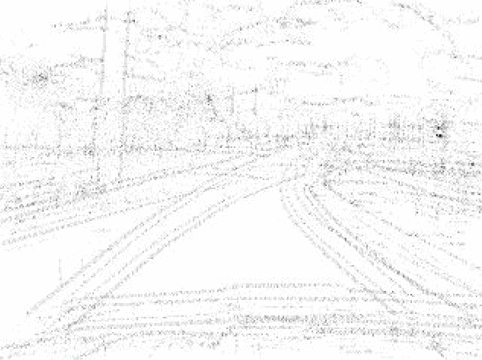
\includegraphics[width=6cm]{img/znaki2.png}
		\subcaption{\label{fig:znaki2}}
	\end{subfigure}
	\begin{subfigure}{0.35\textwidth}
		\centering
		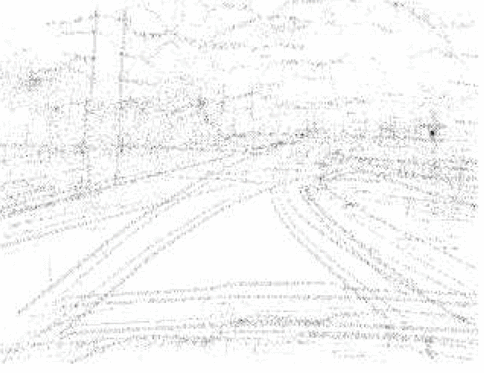
\includegraphics[width=6cm]{img/znaki3.png}
		\subcaption{\label{fig:znaki3}}
	\end{subfigure}
	
	\caption{\label{fig:details}Wyniki detekcji, gdy zakres promieni jest zbyt mały \protect\subref{fig:znaki2} i zbyt duży \protect\subref{fig:znaki3}.\cite{T2}}
\end{figure}

Wszystkie opisywane operacje są wykonywane na obrazach dyskretnych, więc przestrzeń możliwych długości promieni jest skwantowana. W przypadku, gdy dobrany zakres długości promieni będzie zbyt mały lub zbyt duży, detektor ma gorszą sprawność. Dzieje się tak, ponieważ ewentualne maksima są rozmyte (rys. \ref{fig:znaki2} i rys. \ref{fig:znaki3})
%TODO Brak opisu tych rysunków. OK 
%TODO Brak opisu rozwiązania "konkurencyjnego".
%TODO Swoją drogą komentarz co dla innych znaków.

\subsection{Detekcja sygnalizacji świetlnej}
\label{sec:tl}
Kolejnym istotnym elementem systemów umieszczanych w pojazdach autonomicznych jest detekcja świateł drogowych.
%TODO tak się zastanawiam i nie wiem czy światła drogowe to dobra nazwa. Może sygnalizacja świetlna. Bo światła drogowe to w samochodach OK
Informują one o możliwości przejazdu przez skrzyżowanie lub rondo lub opcji znalezienia się na trasie kolizyjnej w stosunku do innych użytkowników drogi. %TODO powt. możliwości OK
Sygnalizacja świetlna spotykana jest głównie w miastach, lecz wraz z rozwojem infrastruktury widywana są także w~mniejszych miejscowościach. 
Słupy z zamontowanymi światłami mogą być widoczne na prawej lub lewej krawędzi jezdni, a także nad nią.

\subsubsection{Detekcja sygnalizacji świetlnej z użyciem informacji o kolorze i krawędziach}

Sygnalizacja świetlna na świecie jest ustandaryzowana. %TODO światła jw. OK
Istnieją trzy kolory: czerwony, żółty i zielony. 
Każdy kolor niesie za sobą informację: czerwony -- stój, żółty -- przygotuj się do zmiany z zielonego na czerwony lub odwrotnie i~zielony, który oznacza jedź. 
Jedyną znaną różnicą w stosunku do opisanego standardu jest światło pomarańczowe, występujące jako zamiennik światła żółtego w Stanach Zjednoczonych %TODO zdanie niejasne OK

\begin{figure}
  \centering
  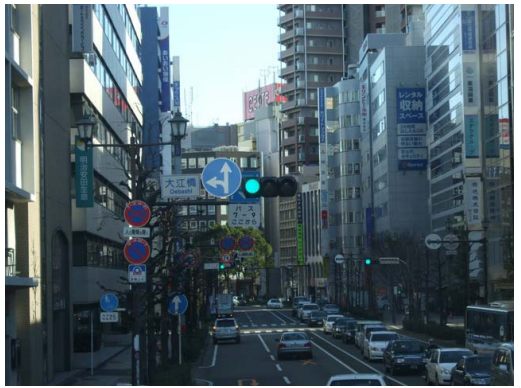
\includegraphics[width=7cm]{img/tl_input.png}
  \caption{Obraz wejściowy algorytmu detekcji sygnalizacji świetlnej\cite{T4}}
  \label{fig:tl_input}
\end{figure}

Masako Omachi w artykule \cite{T4} proponuje algorytm, który bazuje na informacji o kolorze i~krawędziach znajdujących się na obrazie. 
Światła drogowe mają z góry ustalony kształt -- są okrągłe. 
Istnieją warianty ze strzałkami, lecz opisywany poniżej algorytm służy do detekcji świateł, które w \cite{Kodeks} mają kształt pełnego koła.

Rysunek \ref{fig:tl_input} pokazuje przykład sceny zawierającej światła drogowe. 
W~opisywanej metodzie przestrzeń barw jest konwertowana do znormalizowanej przestrzeni RGB. 
Polega ona na zmapowaniu wartości pikseli do przedziału $[0,255]$,a~także ,,rozsunięciu'' wartości pikseli na obrazie tak, by znajdowały się w całym możliwym zakresie wartości:
\begin{equation}
R=\left\{\begin{matrix}
0, &  s=0\\
\frac{r}{s} & w p.p.
\end{matrix}\right.
\end{equation}
\begin{equation}
G=\left\{\begin{matrix}
0, &  s=0\\
\frac{g}{s} & w p.p.
\end{matrix}\right.
\end{equation}
\begin{equation}
B=\left\{\begin{matrix}
0, &  s=0\\
\frac{b}{s} & w p.p.
\end{matrix}\right.
\end{equation}
gdzie:
\begin{itemize}
\item$r,g,b$ -- składowe czerwona, zielona i~niebieska nieznormalizowanego obrazu,
\item$s = r+g+b$
\item$R,G,B$ -- składowe czerwona, zielona i~niebieska znormalizowanego obrazu.
\end{itemize}


\begin{figure}
  \centering
  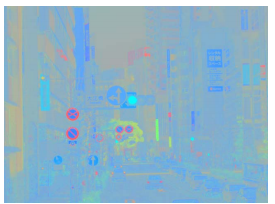
\includegraphics[width=7cm]{img/tl_norm.png}
  \caption{Efekt normalizacji przestrzeni barw\cite{T4}}
  \label{fig:tl_norm}
\end{figure}

Efekt przeniesienia przestrzeni barw do znormalizowanej przestrzeni RGB jest widoczny na rysunku \ref{fig:tl_norm}.
Następnie, poprzez progowanie każdej ze składowych barwnych uzyskuje się obszary, w których mogą znajdować się elementy sygnalizacji świetlnej. %TODO styl. OK
Decyzja o tym czy piksel należy lub nie do elementu sygnalizacji świetlnej jest podejmowana na podstawie poniższych warunków:
\begin{equation}
R>200 \wedge G< 150 \wedge B<150
\end{equation}
lub
\begin{equation}
R>200 \wedge G> 150 \wedge B<150
\end{equation} 
lub
\begin{equation}
R<150 \wedge G>240 \wedge B>220
\end{equation}.

\begin{figure}
  \centering
  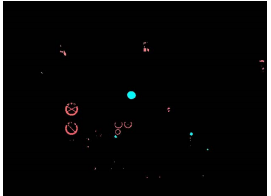
\includegraphics[width=7cm]{img/tl_thresh.png}
  \caption{Rezultat progowania w celu wykrycia obszarów będących kandydatami do bycia sygnalizacją świetlną\cite{T4}}
  \label{fig:tl_thresh}
\end{figure}

Rezultat progowania jest widoczny na rysunku \ref{fig:tl_thresh}. 
Następnym krokiem jest wykrycie krawędzi na obrazie z kandydatami do detekcji świateł. 
Jedną z~opcji jest użycie filtru Sobela. 
Ostatnim etapem, jako że światła drogowe mają jasno określony kształt, jest użycie transformaty Hougha dla okręgów, by wykryć właściwe elementy sygnalizacji świetlnej. 
W~artykule stosowana jest zmodyfikowana transformata Hougha do wyszukiwania okręgów, która polega na ustaleniu stałej długości promienia. 
Klasyczna transformata Hougha jest opisana w podrozdziale \ref{sec:vision_algs}. %TODO sekcji ! OK

%\subsection{Wnioski i rezultaty} %TODO to nie powinno być osobne, bo dotyczy tego samego algorytmu. OK

Opisany algorytm detekcji świateł drogowych daje lepsze wyniki niż użycie standardowej przestrzeni barw i klasycznej transformaty Hougha dla okręgów. 
Porównanie jest zamieszczone w tabeli \ref{tab:tl_results}. 
Główną zaletą opisywanej metody detekcji sygnalizacji świetlnej jest fakt, że poprawnie odrzuca ona znaki drogowe, które również mają okrągły kształt i jednolite kolory na krawędziach. %TODO słowo "obrazy" nie pasuje OK
Kolejnym sprawdzanym elementem jest kolor na krawędziach, który powinien być taki sam jak wewnątrz kształtu, co pozwala skutecznie odrzucić np. znaki zakazu. %TODO "bierze" - personifikacja OK
Problemem, który napotyka algorytm są tylne światła innych pojazdów, które mają jednolity kolor (z reguły czerwony), a także kształt zbliżony do czerwonego światła sygnalizatora. %TODO kształt ? OK
Przykładowy błąd detekcji jest ukazany na rysunku \ref{fig:tl_err}.

\begin{figure}
  \centering
  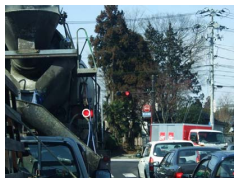
\includegraphics[width=7cm]{img/tl_err.png}
  \caption{Przykład błędnej detekcji tylnego światła traktora\cite{T4}}
  \label{fig:tl_err}
\end{figure}

\begin{table}[]
\centering
\caption{Porównanie klasycznego algorytmu detekcji świateł i opisanego w pracy\cite{T4}} %TODO W pracy X OK
\begin{tabular}{lllll}
\cline{1-3}
\multicolumn{1}{|l|}{}                           & \multicolumn{1}{l|}{Algorytm klasyczny} & \multicolumn{1}{l|}{Algorytm opisany w tym rozdziale} &  &  \\ \cline{1-3}
\multicolumn{1}{|l|}{Dokładność}                 & \multicolumn{1}{l|}{20/30}              & \multicolumn{1}{l|}{26/30}                            &  &  \\ \cline{1-3}
\multicolumn{1}{|l|}{Czas przetwarzania {[}s{]}} & \multicolumn{1}{l|}{0.561}              & \multicolumn{1}{l|}{0.347}                            &  &  \\ \cline{1-3}
                                                 &                                         &                                                       &  & 
\end{tabular}
\label{tab:tl_results}
\end{table}
%TODO a to co jest alg. klasyczy.

%TODO konkurencyjna metoda
%TODO NN - są fajnie prace, łatwo Pan znajdzie.



\subsection{Detekcja samochodu poprzedzającego}
\label{sec:car_general}

Istotnym zadaniem stawianym przed algorytmami wizyjnymi stosowanymi w~pojazdach autonomicznych jest wykrycie samochodów w najbliższym otoczeniu pojazdu. 
Detekcja może być wspierana odczytami z radaru lub lidaru, jednak w~poniższym podrozdziale zostanie opisany algorytm bazujący jedynie na obrazie z kamery. %TODO 1. powt. detekcja, sekcja !, kamery, czy kamer OK, kamery, są algorytmy, które składają obraz z dwóch kamer, ale faktycznie opisywany alg. korzysta z jednej
Większość współczesnych samochodów widzianych od tyłu zachowuje symetrię względem pionowej osi przechodzącej przez środek pojazdu. 

Pierwszym, wstępnym krokiem jest zbadanie możliwych pozycji samochodów na obrazie i oznaczenie ich jako ROI.
Dla systemu z~fuzją danych wizyjnych i radarowych może to być zrobione poprzez analizę odległości i prędkości względnej, czyli danych uzyskanych z radaru. 
Dla systemu, który posiada jedną kamerę, pozycja samochodów musi być wyznaczona tylko na podstawie ruchu samochodów na obrazie w czasie.

Opisywany algorytm korzysta z detektora symetrii, który działa w następujący sposób. 
Dla każdego piksela wyznaczana jest liczba punktów, która jest wartością bezwzględną z różnicy wartości pikseli, które są równoodległe od ustalonej osi symetrii(równanie {eq:sym_detect}). %TODO niejasne - rysunek - dałem odnośnik do równania w dalszej części tekstu, które lepiej obrazuje sposób działania detektora
Jest to zwykle robione z użyciem pewnego okna o z góry ustalonym rozmiarze dobieranym tak, aby pasować do rozmiaru samochodów, które mogą znajdować się na obrazie. 
Będąc świadomym faktu, że samochód im jest dalej od kamery, tym jest mniejszy zastosowano kilka predefiniowanych rozmiarów okien. 
Wartości wskaźnika symetrii mogą być obliczane dla każdego punktu na obrazie. 
Piksele z dużą wartością tego wskaźnika są kandydatami do należenia do osi symetrii. %TODO styl. OK
Wyliczanie wskaźnika symetrii dla każdego punktu na obrazie jest bardzo czasochłonne. Zdecydowano się na jego wyznaczanie tylko na wcześniej określonych poziomych liniach, które pokrywają obszar, na którym mogą znajdować się samochody. %TODO styl. na dwa zdania i zgrabniej OK
Do obliczania wskaźnika symetrii może być użytych kilka cech obrazu takich jak: wartości pikseli w skali szarości, obraz krawędzi, składowa S w przestrzeni barw HSV. 
Szukanie obrazu samochodu na obrazie w skali szarości jest szybsze, jednak wrażliwe na zmiany oświetlenia (noc, deszcz). 
Dobrze sprawdza się badanie nasycenia w przestrzeni barw HSV, ponieważ uniezależnia to obraz samochodu od ogólnej jasności otoczenia i~częściowo od pogody.

\subsubsection{Przebieg algorytmu bazującego na operatorze symetrii}
%TODO To całe to powinnien być podrodział, a to ew. subsub lub paragraph.
Pierwszym krokiem jest wygenerowanie obrazu krawędzi na podstawie obrazu w skali szarości lub składowej S przestrzeni barw HSV. 
W~opisanym algorytmie zaproponowano detektor Canny'ego. 
Rysunek \ref{fig:car_edge} pokazuje rezultat wykrywania krawędzi dla typowego obrazu zawierającego samochód poprzedzający. 
Opierając się na znanej pozycji kamery i jej pochyleniu względem nawierzchni drogi można określić obszar na obrazie, na którym będą szukane samochody. 
Poziome ograniczenia znajdują się pomiędzy horyzontem i początkiem widocznej drogi na dole obrazu. 
Pionowe ograniczenia są ustawione tak, by odpowiadać lewemu i prawemu ograniczeniu jezdni. 

\begin{figure}
  \centering
  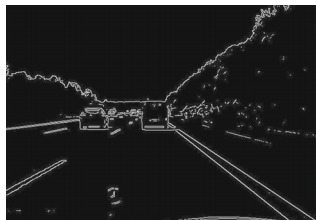
\includegraphics[width=7cm]{img/car_canny.png}
  \caption{Obraz z samochodami po filtracji filtrem Canny'ego\cite{T1}}
  \label{fig:car_edge}
\end{figure}

Jak wspomniano w sekcji \ref{sec:car_general}, w celu zredukowania czasu obliczeń nie każdy piksel w wybranym obszarze jest analizowany. 
Obliczenia dotyczące symetrii są przeprowadzane tylko dla 15 równoodległych linii skanu (rys. \ref{fig:car_scan_lines1}). 
Wejściowa rozdzielczość obrazu nie ma znaczenia dla obliczeń. %TODO no pozioma jednak ma.... - chodzi o to, że obraz może być przeskalowany do pewnej założonej rozdzielczości.
Dzieje się tak ponieważ algorytm wykrywa tylko maksima wzdłuż linii skanu. Autorzy algorytmu zalecają przeskalowanie obrazu do niższej rozdzielczości w celu zredukowania czasu przetwarzania.

\begin{figure}
  \centering
  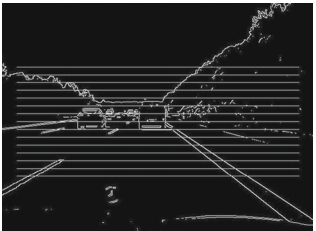
\includegraphics[width=7cm]{img/car_lines.png}
  \caption{Obraz z samochodami po filtracji filtrem Canny'ego i zaznaczonymi liniami skanu\cite{T1}}
  \label{fig:car_scan_lines1}
\end{figure}

Kolejnym krokiem jest detekcja symetrii. 
Jest ona przeprowadzana dla każdego punktu leżącego na linii skanu.
Wartość operatora symetrii dla piksela wyraża się wzorem:

\begin{equation}
\label{eq:sym_detect}
SymVal(x,y)=\sum_{x'=1}^{W/2}\sum_{y'=y-H/2}^{y+H/2}S(x, x', y')
\end{equation}
gdzie:
\begin{itemize}
\item
\begin{equation}
S(x,x',y')=\begin{cases}
2 & \text{ gdy } I(x-x',y')=I(x+x',y')=1 \\ 
-1 & \text{ gdy } I(x-x',y')\neq I(x+x',y') \\ 
0 & \text{ w p.p. }
\end{cases}
\end{equation}
\item $W$ -- szerokość okna
\item $H$ -- wysokość okna
\item $I(x,y)$ -- wartość piksela o współrzędnych $x,y$
\end{itemize}

Szerokość okna powinna być właściwie ustawiona, aby poprawnie wykrywać symetryczne obiekty o różnych rozmiarach. 
W~trakcie eksperymentów wykazano, że wartości dające poprawne rezultaty $W$ mieszczą się w przedziale $[8,12]$. %TODO optymalne...to nie dobre słowo po AiR w tym kontekście. OK - ciężko znaleźć właściwy wskaźnik jakości

\begin{figure}
  \centering
  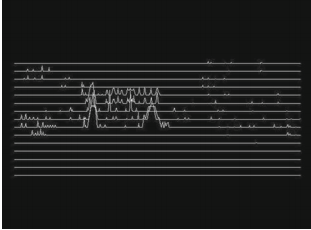
\includegraphics[width=7cm]{img/tl_peaks.png}
  \caption{Wartości wskaźnika symetrii wyznaczone dla linii skanu\cite{T1}}
  \label{fig:car_scan_lines}
\end{figure}

Na rysunku \ref{fig:car_scan_lines} widać, że w niektórych punktach istnieją maksima, które wskazują, że dany punkt może należeć do osi symetrii. 
W kolejnym kroku wybiera się maksima i stosuje progowanie, to znaczy wartości maksimów lokalnych poniżej pewnej wartości są odrzucane. %TODO W kolejnym kroku... OK
Zwykle wartości poniżej określonego progu wskazują na małe, symetryczne elementy tła. 
Progowanie dokonuje się według następującej formuły:
\begin{equation}
SymPts(x,y)=\begin{cases}
1 & \text{ gdy } SymVal(x,y)>T\\ 
0 & \text{ w p.p.}
\end{cases}
\end{equation}

gdzie:
\begin{itemize}
\item $T$ - ustalony próg odrzucenia maksimum lokalnego
\end{itemize}


\begin{figure}
  \centering
  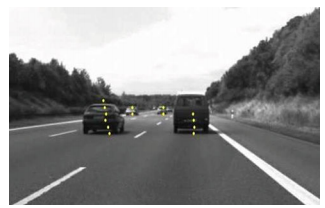
\includegraphics[width=7cm]{img/car_symmetry.png}
  \caption{Wykryte osie symetrii na liniach skanu\cite{T1}}
  \label{fig:car_detected}
\end{figure}

Ostatecznie znalezione maksima oznaczają wykryte osie symetrii względnie dużych obiektów, w tym przypadku samochodów. 
Widać to na rysunku \ref{fig:car_detected}. 
Dla każdej linii skanu wykryta oś symetrii jest przesunięta o kilka pikseli, dlatego ostatnim etapem detekcji samochodu jest klasteryzacja.

Uzyskane punkty osi symetrii są klasteryzowane metodą k-średnich. 
Liczba samochodów na obrazie jest nieznana, więc klasteryzację przeprowadza się iteracyjnie, co iterację licząc wariancję, która przy poprawnej liczbie klastrów w stosunku do samochodów na obrazie będzie mniejsza niż określony próg. 
Końcowy wynik z zaznaczonymi środkami samochodów jest widoczny na rysunku \ref{fig:car_end}

\begin{figure}
  \centering
  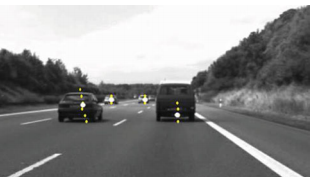
\includegraphics[width=7cm]{img/car_end.png}
  \caption{Wynik algorytmu detekcji samochodów poprzedających\cite{T1}}
  \label{fig:car_end}
\end{figure}

%TODO drugie podejście
%TODO podejście NN

%TODO Proszę już nie dopisywać osobnego rodziału, ale gdzieś wspomnieć np. o detekcji pieszych, czy rowerzystów...


\section{Opis wybranych zagadnień i algorytmów przetwarzania obrazu}
\label{sec:vision_algs}
W tym podrozdziale zostaną opisane podstawowe algorytmy i zagadanienia dotyczące cyfrowego przetwarzania obrazów, które są używane w zaawansowanych algorytmach wizyjnych w pojazdach autonomicznych. %TODO "sekcja". OK

\subsection{Transformata Hougha dla okręgów}

Systemy wizyjne w pojazdach autonomicznych często mają za zadanie wykrycie obiektów o kształcie koła. Algorytmem do tego przeznaczonym jest transformata Hougha. 
Istnieje ona w wersji do detekcji prostych i okręgów. 
Pod pojęciem uogólniona transformata Hougha należy rozumieć algorytm służący do detekcji dowolnego zadanego konturu.
%TODO "kryje się" zły styl OK

Okrąg można sparametryzować za pomocą następującego wzoru:
\begin{equation}
(x-x_0)^2+(y-y_0)^2=r^2
\end{equation}
gdzie:
\begin{itemize}
\item $x_0, y_0$ -- współrzędne środka okręgu,
\item $r$ -- promień okręgu.
\end{itemize}

\begin{figure}[h]
\centering
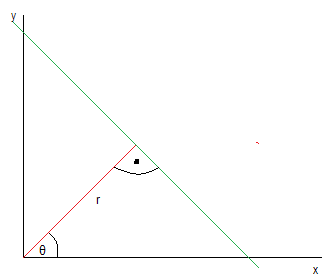
\includegraphics[width=7cm]{img/hough.png}
\caption{Linia w układzie współrzędnych określona za pomocą parametrów $(r, \theta)$}
\label{fig:hough}
\end{figure}
%TODO brak odniesienia w txt

Jeżeli promień będzie ustalony, to okrąg zostanie sparametryzowany za pomocą dwóch liczb. 
Gdy szukamy okręgów o nieznanych promieniach, rośnie złożoność obliczeniowa, ponieważ wymiar przestrzeni parametrów zwiększa się o jeden.

Możliwa jest również parametryzacja okręgu w biegunowym układzie współrzędnych (rys. \ref{fig:hough}):
\begin{equation}
x = x_0 + rcos(\theta)
\end{equation}
\begin{equation}
y = y_0 + rsin(\theta)
\end{equation}

po prostym przekształceniu otrzymuje się:

\begin{equation}
x_0 = x - rcos(\theta)
\end{equation}
\begin{equation}
y_0 = y - rsin(\theta)
\end{equation}

Następnie wyznaczana jest przestrzeń Hougha. W niej akumulowane są wartości oznaczające liczbę okręgów, które przechodzą przez dany piksel na obrazie wejściowym. Ten proces nazywa się głosowaniem. 
Wartości maksymalne w przestrzeni Hougha oznaczają wykryty okrąg.

%TODO brakuje wyjaśnienia jak działa ta przestrzeń Hougha OK

\subsection{Przestrzenie barw}

Podstawową przestrzenią barw jest RGB. 
Przestawiona jest na rysunku \ref{fig:rgb} za pomocą sześcianu. 
Każda składowa jest odpowiedzialna za informację o zawartości danego koloru. 
Jej zaletą jest prostota opisu, natomiast wadą jest fakt, że po niewielkiej zmianie wartości składowych otrzymuje się zupełnie inną barwę. 
Dodatkowo, co jest ważne w przypadku systemów wizyjnych, niewielka zmiana poziomu jasności powoduje duże wahania składowych R, G, B.

\begin{figure}
  \centering
  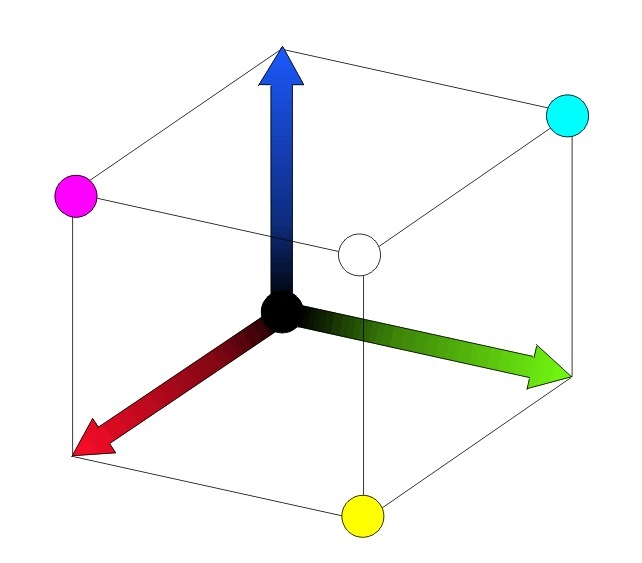
\includegraphics[width=7cm]{img/rgb.jpg}
  \caption{Sześcian przedstawiający przestrzeń barw RGB\cite{W4}}
  \label{fig:rgb}
\end{figure}


\begin{figure}
  \centering
  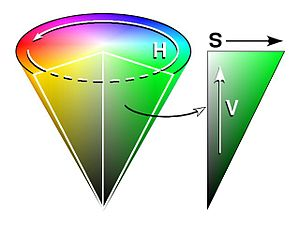
\includegraphics[width=7cm]{img/hsv.jpg}
  \caption{Stożek przedstawiający przestrzeń barw HSV(\textit{źródło: Wikipedia})}
  \label{fig:hsv}
\end{figure}

Drugą, ważną przestrzenią barw używaną w cyfrowym przetwarzaniu obrazów jest przestrzeń HSV. 
Jest ona przedstawiona na rysunku \ref{fig:hsv} za pomocą stożka. 
Jej główną zaletą jest to, że przy niewielkich zmianach jasności zauważalne są niewielkie zmiany składowej S. %TODO styl. OK
Pozwala to na uniezależnienie się w pewnym stopniu od czynników takich jak pora dnia lub pogoda.

\subsection{Filtr Canny'ego}
Podstawowym, dobrze sprawdzającym się detektorem krawędzi, jest filtr Canny'ego \cite{T5}. 
Cechuje się następującymi właściwościami: %TODO by se przydało źródło (choćby oryginalny artykuł Cannego) OK

\begin{itemize}
\item niska liczba fałszywych detekcji krawędzi,
\item poprawne wskazywanie pozycji krawędzi. Pozycja krawędzi wskazywana przez detektor powinna odpowiadać jej prawdziwemu położeniu
\item jedna wykryta krawędź przypadająca na rzeczywistą krawędź
\end{itemize}

Detektor krawędzi Canny'ego jest algorytmem wieloetapowym:
\begin{enumerate}
\item Redukcja szumów z obrazu. Używany jest filtr Gaussa. Przykładowa macierz filtru pokazana jest na rysunku \ref{fig:canny_gauss}. %TODO to jakichkolwiek to przesada - redukcja szumu OK
\begin{figure}[h]
\centering
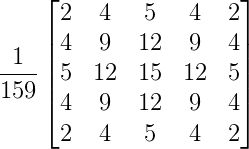
\includegraphics[scale=0.8]{img/canny_gauss.png}
\caption{Maska filtru Gaussa stosowana w wykrywaniu krawędzi}
\label{fig:canny_gauss}
\end{figure}
\item Wyszukiwanie krawędzi z użyciem filtru Sobela o poziomej i pionowej orientacji.
\item Określenie wartości gradientu i jego kierunku:

\begin{equation}
G=\sqrt{G_x^2+G_y^2}
\end{equation}

\begin{equation}
\theta=arctan(\frac{G_y}{G_x})
\end{equation}
Kierunek jest kwantyzowany na jeden z czterech możliwych kierunków: \ang{0}, \ang{45}, \ang{90}, \ang{135}.
%TODO może lepiej kwantyzowany ? OK

\item Wartości gradientu w kierunku prostopadłym do głównego przebiegu wykrytej krawędzi o niemaksymalnych wartościach są usuwane. %TODO dodać w jakim otoczeniu OK
Ma to na celu usunięcie pikseli, które prawdopodobnie nie są elementem krawędzi. 
W wyniku tej operacji pozostają tylko cienkie linie jako krawędzie.

\item Filtr Canny'ego jako argumenty otrzymuje dwa progi -- górny i dolny:
\begin{itemize}
\item jeżeli wartość gradientu przekracza górny próg, piksel jest zawsze uznawany jako krawędź,
\item jeżeli wartość gradientu nie przekracza dolnego progu, piksel nie jest uznawany za krawędź,
\item jeżeli wartość gradientu jest pomiędzy dwoma progami, jest krawędzią, tylko wtedy gdy jest połączony z pikselem, który został sklasyfikowany jako krawędź.
\end{itemize}
Twórca filtru rekomenduje stosunek progów filtru pomiędzy 2:1 i 3:1
\end{enumerate}